\documentclass[MasterThesisMain.tex]{subfiles}
\begin{document}
\chapter{Discussion} \label{ch:discussion}

\section{Experimental setup}
The experimental setup can be used in two ways. The first way with the optical fiber in the single point stage and the second way with the optical fiber in the solvent vapour annealing chamber. When the optical fiber is fitted into the solvent vapour annealing chamber, the light must pass through a sapphire lens. This causes a great deal of reflected light and affects the reflectance measurements taken. This can be seen by holding the static measurements seen in table \ref{tab:polymers} against the first fitted thickness values found in the figures for each polymer in chapter \ref{ch:results}. The effects may be small at the beginning of the solvent vapour annealing when the polymer has not swelled, but during swelling the reflectance measurements drop and can be zero in some intervals. The sapphire lens effectively increases the dark measurement and when calculating the reflectance, since the dark measurement is in the denominator, lowers the reflectance measurements. It can be seen when plotting the reflectance measurements alone with no strict axis interval that some of the reflectance measurements drop below zero, as seen in figure \ref{fig:drop}. The reason for this is unknown. Reflectance measurements close to zero can be seen in figure \ref{fig:drop2}. The dark measurements are taken when the optical fiber is fitted into the solvent vapour annealing chamber with a piece of black fabric where the wafer would lie. The black fabric is a piece of black cotton. The effect, if there is any, of the black fabric has not been investigated. The distance from the wafer to the optical fiber is important, as it is seen to shift the whole reflectance measurement up and down the y axis. Up if the distance increases and down if it decreases. It is therefore very important to use a step wafer where the thickness is known, to adjust the single point stage before a static measurement of a wafer with a thin film. When the optical fiber is placed in the solvent vapour annealing chamber, the distance between the optical fiber and the wafer is much greater than it is intended, and the sapphire lens is used to focus the light to illuminate the wafer. Calibrating the solvent vapour annealing setup is impossible since the chamber is not big enough for the step wafer to be placed in the chamber. Taking the best reference and dark measurement is key to a good reflectance measurement for the thin film, although it seems that the most precise measurement is impossible. A measurement close to precise can be achieved as seen in the fitting of the Fresnel equations using the homopolymers reflectance data.

\begin{figure}[H]
\centering
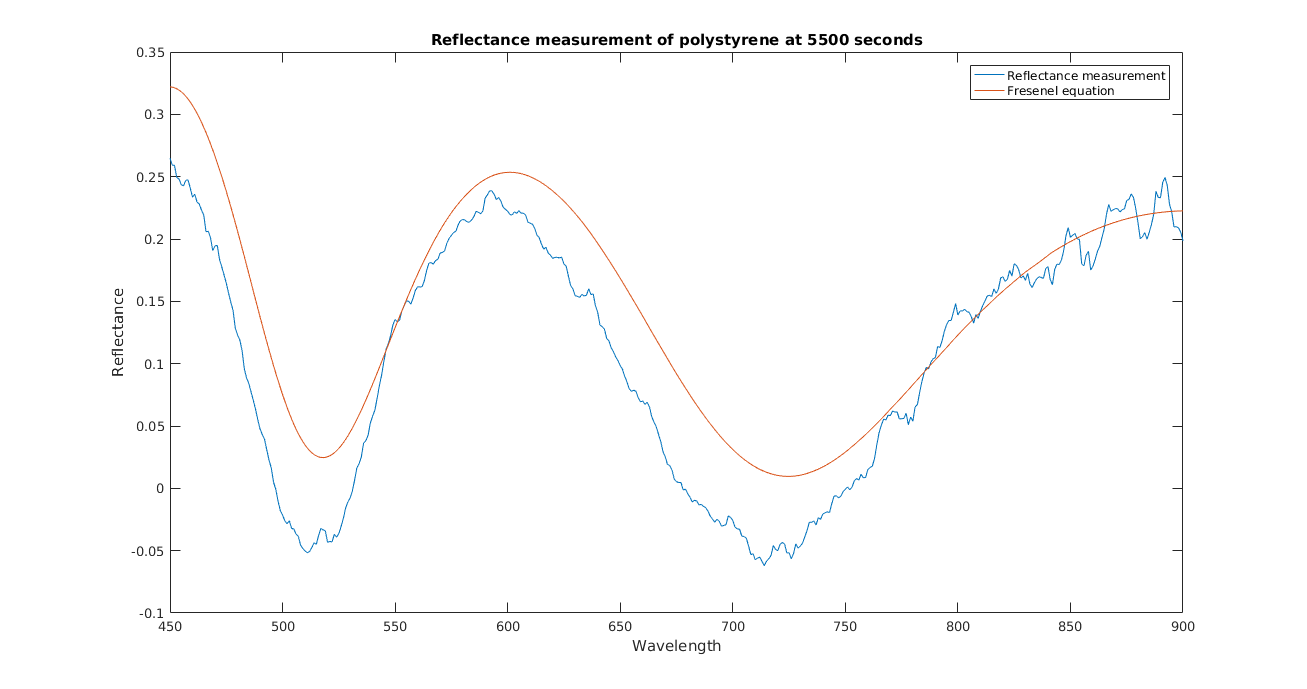
\includegraphics[width = \textwidth]{refldrop.png}
\caption{The reflectance measurement for polystyrene at time $5500$ seconds with the best fitting fresnel equation plotted. It can be seen that the reflectance measurement drops compared to the theoretical model. The cause for the drop in the reflectance measurement is unknown. The drop in the reflectance measurement affects the mean square error fitting, increasing the mean square error during the swelling.}
\label{fig:drop}
\end{figure}

\begin{figure}[H]
\centering
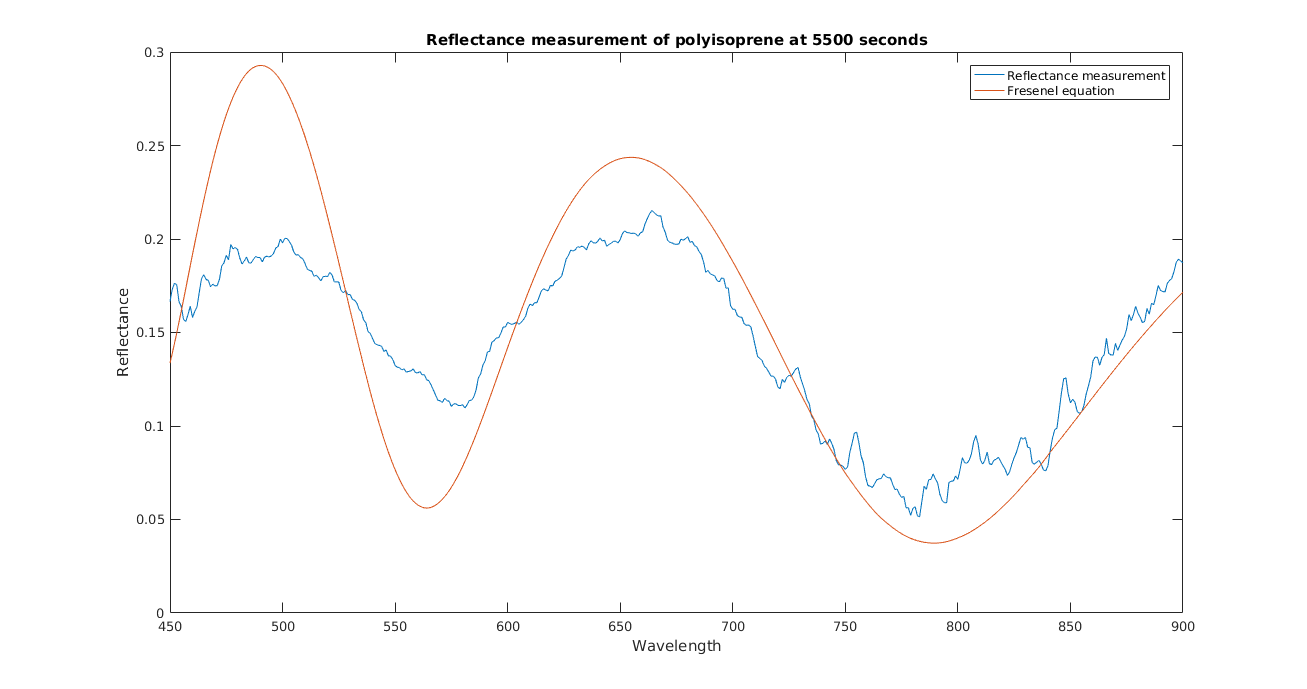
\includegraphics[width = \textwidth]{refldrop2.png}
\caption{The reflectance measurement for polyisoprene at time $5500$ seconds with the best fitting Fresnel equation plotted. It can be seen that the reflectance measurement drops compared to the theoretical model. The cause for the drop of amplitude in the reflectance measurement is unknown. The drop of amplitude in the reflectance measurement affects the mean square error fitting, increasing the mean square error during the swelling. The general form of the reflectance measurement can be seen in the fitting, where the peaks and the valleys of both curves match.}
\label{fig:drop2}
\end{figure}

\section{Refractive index dispersion of polymers and absorption}
The refractive index dispersion of the polymers has been shown in figure \ref{fig:dispshort} using the values given by the experimental method ellipsometry. It can be seen that the refractive index varies across the wavelengths. Polystyrene's refractive index does not vary as greatly as polyisoprene and polystyrene-b-polyisoprene. The fitting has not taken into account the dispersion of the refractive index, instead the constant refractive index has been used. It is unknown how the uptake of the solvent would effect the dispersion and how the dispersion would effect the reflectance measurements. An analytical study of the Fresnel equations would be needed to fully grasp how changing the refractive indices impact the reflectance curves. Absorption is another parameter that can affect the reflectance measurements. Absorption is not present in the Fresnel equations and can be the cause for the divergence between the reflectance measurements and the Fresnel equations. 

\section{Refractive index of toluene vapour}   
The conclusion of the solvent vapour annealing ambient study was that during the solvent vapour annealing protocol the ambient increases from $1$ to $1.3$. The ambient starts off as air with a refractive index of $1$ and as the toluene vapour starts to fill the chamber, the air and the toluene vapour mix. The refractive index of $1.3$ seems reasonable for the toluene vapour. My argument for this is that vapour is in a gas state below its critical temperature but can liquefy due to an increase in pressure. The refractive index for toluene in a liquid state is $1.496$ \cite{toluene}. The refractive index of toluene vapour cannot be greater than the refractive index for toluene in a liquid state, so the vapour refractive index must bounded by an interval spanning $1$ to $1.496$. When swelling, there is a possibility that condensation forms in the chamber. This has not been investigated.  

\section{Mean square error fitting}
The mean square error fitting has been used as it was the fitting protocol used in the Nano-Calc software, and other fitting methods have not been studied or implemented. The interval of fitting has been chosen to run from $\SI{450}{\nano\meter}$ to $\SI{900}{\nano\meter}$. This interval has been the easiest to fit to due to the reflectance measurements being smooth in this region. The fitting of the reflectance measurements follow the features seen in the Fresnel equation, but when swelling commences, the reflectance measurements shift and drop. This can be seen in the figures \ref{fig:drop} and \ref{fig:drop2}. Both figures have been taken at the $5500$ second mark, at the end of the max swelling interval and the reflectance measurements have shifted and dropped with respect to the theoretical model. The way the fitting has been implemented into matlab can also be critiqued. The fitting loads a reflectance measurement and loops through the refractive indices for air and the thin film and the thickness values. For polystyrene this amounted to $13,380,120$ combinations taking roughly $75$ minutes to loop through, for polyisoprene $8,116,164$ combinations taking roughly $44$ minutes and polystyrene-b-polyisoprene $2,462,592$ combinations roughly $13$ minutes. The fitting on the two homopolymers show results that are in accord with what is expected. As the nitrogen flows through the toluene solvent, the toluene vapour increases in the chamber and the refractive index for the ambient increases. This can also be seen for the refractive index of the thin films, as I expect solvent uptake. The thickness values increase as well, marking the point when the solvent vapour annealing protocol has increased and decreased the channels. 

The ambient refractive index is normally set to $1$ when making static measurements. During the ambient study, the reflectance measurements show a decrease during swelling. The fitting increases the refractive index for the ambient and the Fresnel equations follow the reflectance measurements well. The increases in the mean square error values for the ambient study can be caused by the large step sizes in the refractive index. The step size used in the  fitting have been set crudely. The step size for the thickness is set to $1$. Since we are working on the nanoscale, having thickness values with decimals does not shine light on anything interesting when looking at the thickness measurements. The step size for both refractive indices has been set to $0.1$. This has been set to one decimal for two reasons. The first reason is that the more values the fitting has to loop through, the longer the fitting will take, and the second reason is that a finer step size would not contribute useful information to the thickness fitting. What is important is that there is an increase.        

\section{Solvent vapour annealing}
In the solvent vapour annealing protocol, the nitrogen flow has been set to be constant through out the protocol. The assumption is that holding the flow constant will hold the vapour pressure in the chamber constant. This is a crude assumption since the variables flow and pressure are heavily dependant on the tube sizing, the volume of the solvent vapour annealing chamber, the volume of the bubbler and the volume of liquid present in the bubbler. Taking these variables into account and calculating the vapour pressure constitutes a research project in itself. The solvent vapour annealing protocol has been programmed into a script which the mass flow controllers software could read and run. As seen in figure \ref{fig:slowslow}, the increases and decreases of flow controlled by the mass flow controllers happen before they should. Each step apart from the maximum swelling should have a length of $1000$ seconds. The solvent vapour annealing time file was not saved, so I can not precisely determine when the mass flow controllers changed the flow, but the solvent vapour annealing protocol was close to what was scripted.   

\section{Polystyrene and Polyisoprene}
When fitting the Fresnel equations using the reflectance measurements, the homopolymer results behaved as anticipated, but the diblock copolymer results were the opposite of what was expected. The expected results were an increase in ambient refractive index and thin film refractive index which coincided with the increase of toluene vapour present in the chamber. What I expected with the thickness results was an increase in thickness, starting every time there was an increase of toluene vapour. These expectations of how the results should look were met. The thickness results show a 'shark dorsel fin' during the maximum swelling region. One can think that if the maximum swelling was left to continue, the thickness would reach a constant value. There is an interval of time between a change from the mass flow controllers to the beginning of a change in the polymers, which is called a response time. [ADD Values]. The mean square error for both the polystyrene and polyisoprene show a constant mean square error except for when the maximum swelling commences. This is because the fit and the reflectance data do not match up. In figure \ref{fig:drop}, it can be seen that the fit for polystyrene is higher than the polystyrene reflectance measurement. In figure \ref{fig:drop2}, the amplitude of the polyisoprene fit is much greater that the polyisoprene reflectance measurement. During the swelling it is apparent that something is happening that the Fresnel equations do not account for. This could be a multitude of things since the Fresnel equations are simple. The Fresnel equations do not account for an inhomogeneous increase in thickness. The Fresnel equations assume a homogenous increase throughout the thin film but since there are thermodynamic forces, interaction forces between the monomers and the spread of vapour in the chamber, the thin film will increase in an inhomogeneous way. The roughness, variations in thickness in the thin film, can play a role as this can cause diffusive reflection and decrease the reflectance measurements. The polystyrene thickness values are erratic in the swelling and the deswelling but steady in the maximum swelling region. The same can be said for polyisoprene's swelling and deswelling, but in the maximum swelling region the polyiosprene thickness drops twice and returns to the maximum thickness again of $\SI{550}{\nano\meter}$. Each drop is roughly $\SI{25}{\nano\meter}$. The drops in thickness could be the polyisoprene rearranging and the sharp drop looks steep because the measurement timescale and the timescale of the polymer do not match. Measurements are taken every 10 seconds, thus the thickness values can be thought of as discrete.

\section{Polystyrene-b-polyisoprene}
The fitting for the diblock copolymer polystyrene-b-polyisoprene behaves strangely. The fitting shows an ambient refractive index starting at $1.2$ and decreasing in value as the toluene vapour increases. The thin film refractive index does not increase until the solvent vapour annealing protocol reaches the region of maximum swelling. In this region the thin film refractive index climbs rapidly and is erratic throughout the maximum swelling. The thickness does increase nicely throughout the solvent vapour annealing protocol. The mean square error is large at the start of the swelling and decreases during the swelling. The mean square error does peak during the swelling, this coincides with the fitting protocol changing the ambient refractive index from $1$ to $1.1$. The fitting implemented has used one layer with a varying real refractive index. This simple model does not capture the actual structure seen with diblock copolymers. Diblock copolymers organises itself into a multilayer system consisting of a layer consisting of the A block and the next layer consisting of the B block, an A-B-A-B thin film structure, which can consist of many layers. This structure is not seen in the homopolymers, as they consist of one monomer repeated. Fitting for this multilayer thin film with my fitting protocol requires a large amount of computer power. When adding a new variable into the protocol, you are effectively multiplying the amount of values the new variable has onto the amount of combination the fitting protocol, increasing the total amount of calculations the fitting protocol has to calculate. The fitting protocol is not suited to diblock copolymers.     

\end{document}